\begin{document}

\chapter{Methodology}

\section{Data Collection and Preprocessing}
The textual data in this study is written text of pre-modern Chinese and present-day Chinese, and obtained from three sources, namely \gls{ctext} \parencite{sturgeon2019ctext}, \gls{asbc} \parencite{chen1996sinica}, and Dcard\footnote{\url{https://www.dcard.tw/}}. The data from the aforementioned sources are sequential in time and large in size, which allows for a diachronic view of how the concept of home evolves. To scale up this line of research, diachronic embeddings will be trained, made more and more possible and in demand as the digitalization of historical texts and online communication.

Firstly, the Chinese Text Project collects ``pre-modern Chinese texts'' with time spanning from 1046 B.C. of the Western Zhou dynasty onward \parencite{sturgeon2019ctext}. Since the number of texts available from each era varies, and given that the higher the number of texts, the more diverse the content, the time frame with the highest number of texts is chosen to construct the sub-corpora of pre-modern Chinese in this study, and the database can be expanded if data of an earlier era is directly followed by data of the next era. As shown in \tref{tab:num_text}, texts from Tang, Song, Yuan, Ming, and Qing dynasties are the largest in size, and are continuous in order, and thus are retrieved from the \gls{ctext} database using ctext, a Python wrapper for the \gls{ctext} Application Programming Interface (API) developed by Dr. Donald Sturgeon.

\begin{table}[H]
    \def\negdiff#1{~(-\SI{#1}{})}
    \centering
    \begin{tabular}{S[table-format=4,group-separator={},table-space-text-post={~-- \SI{9999}{}}]@{\hspace{1ex}}cS[table-format=4]S[table-format=4]S[table-format=4, table-space-text-post={~(\SI{9999}{}})]}
    \toprule
      \multicolumn{2}{c}{Time span (A.C.)} &
      \multicolumn{1}{c}{Number of texts} &
      \multicolumn{1}{c}{Number of unique texts} \\
    \midrule
      \tang & (Tang) & 956 & 623 \negdiff{333}\\
      \song & (Song) & 2998 & 2145 \negdiff{853}\\
      \yuan & (Yuan) & 991 & 742 \negdiff{249}\\
      \ming & (Ming) & 4248 & 3497 \negdiff{751}\\
      \qing & (Qing) & 9669 & 7719 \negdiff{1950}\\
    \cmidrule{1-4}
      \multicolumn{2}{c}{Average} & 3772 & 2945 \negdiff{827}\\
    \bottomrule
    \end{tabular}
    \caption{Data composition of the \gls{ctext} corpus}
    \label{tab:num_text}
\end{table}

\begin{table}[H]
    \centering
    \begin{tabular}{@{}cS[table-format=4,group-separator={},table-space-text-post={~-- \SI{9999}{}}]@{}S[scientific-notation=true,round-mode=places,round-precision=1]@{}S[scientific-notation=true,round-mode=places,round-precision=1]@{}S[scientific-notation=true,round-mode=places,round-precision=1]@{}S[scientific-notation=true,round-mode=places,round-precision=1]@{}}
    \toprule
      \multirow{2}{*}{Corpus} &
      \multicolumn{1}{c}{\multirow{2}{*}{Time span (A.C.)}} &
      \multicolumn{2}{c}{All texts} &
      \multicolumn{2}{c}{Selected texts} \\
    \cmidrule(lr){3-4} \cmidrule(lr){5-6}
      \multicolumn{2}{c}{} &
      \multicolumn{1}{c}{Tokens} &
      \multicolumn{1}{c}{Types} &
      \multicolumn{1}{c}{Tokens} &
      \multicolumn{1}{c}{Types} \\
    \midrule
      \multirow{5}{*}{\gls{ctext}} &
        {Tang} & 104885709 & 12301 & 39192456 & \\
      & {Song} & 449371130 & 17219 & 56955840 & \\
      & {Yuan} & 104568204 & 11926 & 39588055 & \\
      & {Ming} & 175694880 & 15372 & 71167104 & \\
      & {Qing} & 6399099 & 14502 & 83975052 & \\
    \cmidrule{1-6}
      \gls{asbc} &
      \dynastyASBC & 9169622 & 209143 & N/A & N/A \\
    \cmidrule{1-6}
      Dcard &
      \dynastyDcard & 442780 & 48532 & N/A & N/A \\
    \bottomrule
    \end{tabular}
    \caption{Token and type counts of the diachronic corpora}
    \label{tab:token_type_counts}
\end{table}

% The average character type is \num{14200} for the CTEXT Corpus, and \num{67000} for the \gls{asbc}. Following the data composition of \textcite{hamilton2016law}, this study selects top \num{5000} (\percentage{35.21}\%) and \num{25000}  (\percentage{37.31}\%) words by their average frequency as the input textual data to construct time-varying word embeddings.
% fewer than a threshold of 500 times (content-bearing?)
% during model leaning: min_num 10

Secondly, \gls{asbc} contains articles from the year of 1981 to 2007. The total number of segmented word tokens and type in the corpus is 8,940,871 and 66,562 respectively. In addition, not only are articles in \gls{asbc} temporal-labeled, but the texts are also carefully segmented, which makes it an ideal input data for word vector representations. 

The third source of data is Dcard, an online social discussion platform established in December, 2011, in Taiwan. In order to retrieve posts with the most diverse topics Dcard API is utilized to retrieve posts from the section of most lately published articles, rather than posts from a number of selected channels.

Apart from the provision of the API access, the \gls{ctext} project website is informative of how textual data and metadata are stored in the retrieved format. Following the instructions\footnote{\url{https://ctext.org/instructions/wiki-formatting}}, the preprocessing of raw texts is done as described below:

\begin{enumerate}[label={(\arabic*)}]
    \item The raw text is cleaned by (a) removing commentaries and marginal notes, (b) segmenting the text into two levels of chucks to indicate possible sentence and word/phrase boundaries according to the list of punctuations in the Instructions, and (c) extracting Chinese characters encoded in Unicode.
    \item To compile time-sliced subcorpora with equal size and relevant information, only one version is selected. The \gls{ctext} digital library contains multiple versions of a text converted by different OCR (Optical Character Recognition) techniques, and the metadata includes tags that differentiate versions at varying degrees of OCR accuracy. In the case where no tags are provided, the version with the largest file size is selected, which is also the reason why text cleaning preceeds version selection.
\end{enumerate} 

Chinese words are not delimited by space, nor is punctuation systems adopted in pre-modern Chinese text. As a consequence, the punctuations  should be viewed as symbols to mark \zh{句讀}{jùdòu}{pauses or breaks}. Only the symbols specified in the website's instructions are treated as indications of sentence boundaries, namely the newlines, full-width periods (。), and vertical bars (|). During the preprocessing, the set of punctuation marks used for phrase-level segmentation include the CJK Symbols and Punctuations, their half-width counterparts, and variants listed in the Unicode Standard \footnote{\url{https://unicode.org/charts/PDF/U3000.pdf}}.

Unicode range between U+4e00 and U+9fff are retained and used to construct word embeddings.

Text surrounded by quotation marks indicates conversations, sayings, or allusions, and is not removed during the preprocessing. On one hand, conversations are an integral part of the text; on the other, sayings and allusions reveal what is still in use or understandable in the time period of their appearance.

After the completion of preprocessing, this study proceeds to a preliminary quantitative analysis using the R Quanteda library \parencite{quanteda}. Since it is difficult to infer statistically significant frequency changes because linguistic resources of pre-modern Chinese are essentially insufficient and not of good quality, the bootstrapping method proposed by \textcite{lijffijt2016bootstrap} is applied to reduce the influence of uneven distribution of linguistic features in texts and provide a more solid ground for the quantitative analysis. To understand the frequency distribution of characters in a diachronic view, the bootstrapping test is performed with 1K samples of 50 texts from the 500 texts of the Tang and Qing dynasties, as shown in \fref{fig:freq_boot}. 

Specifically, although the relative frequency of \jia slightly increases from \num{1260.92} to \num{1609.15} (The raw frequencies are \num{61420} and \num{1831222}), the difference in the use of the character is not statistically significant: p=0.5404595, 1k samples. Consequently, the use of \jia does not change in frequency, and is regarded as being stable in use.

\begin{figure}[H]
\centering
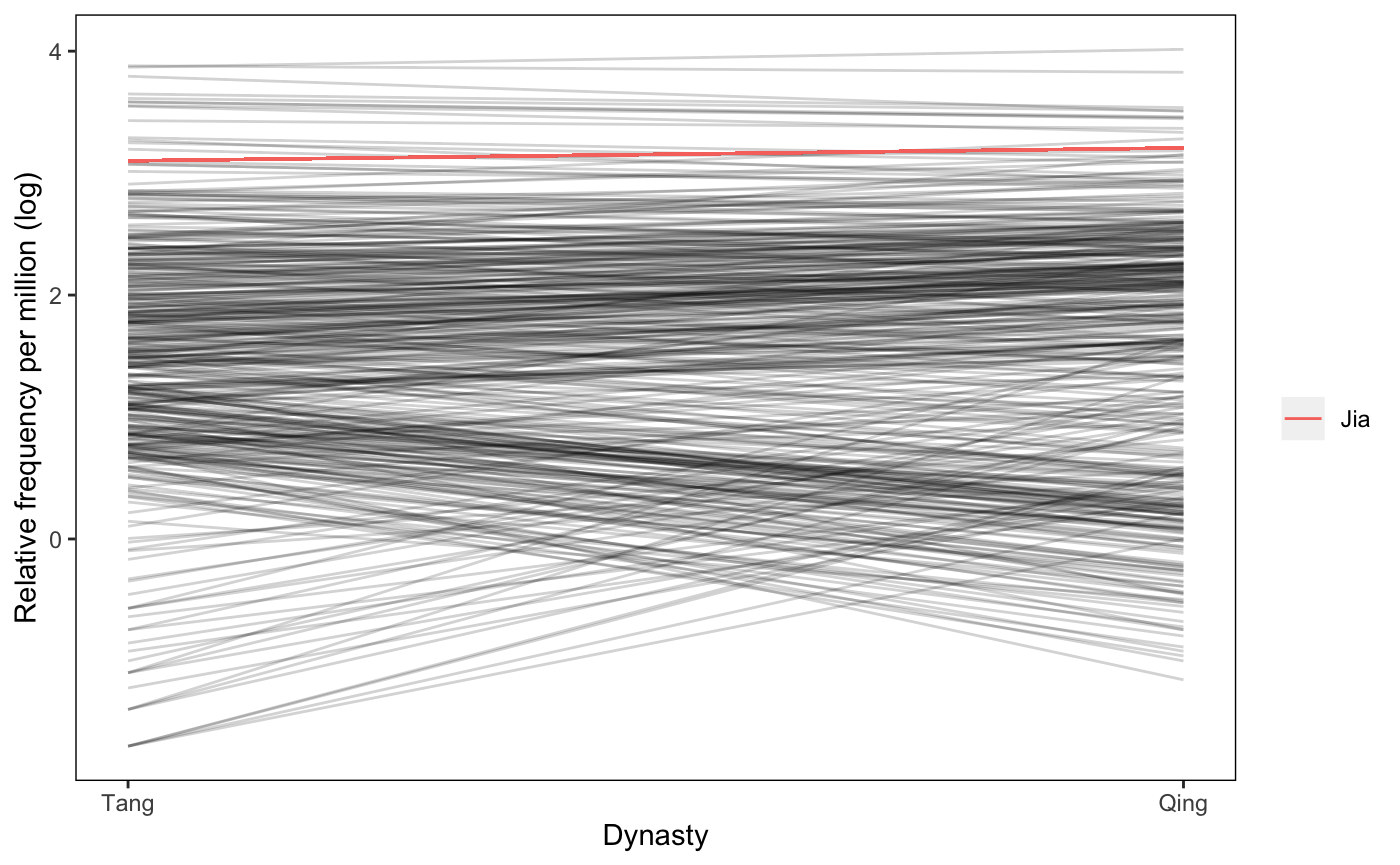
\includegraphics[width=0.75\textwidth,keepaspectratio]{figures/Tang_Qing}
\caption{Frequency change derived from the bootstrapping test on characters between the Tang and Qing dynasty\\\footnotesize{* The line in red represents the frequency change of \jia\rspace.}}
\label{fig:freq_boot}
\end{figure}

Before the degree of semantic change is measured, a filtering of mid-frequency
characters is conducted, for highly frequent characters are not content-bearing \parencite{hamilton2016cultural,rodda2017panta}. Afterwards, the similarity of semantic vectors across time
periods is compared using correlations; namely the similarity between T2 (the time period of
interest) and T1 (the previous time period). Instead of computing on the original vectors,
alternatively called first-order embeddings, we resort to second-order embeddings composed
of a full or partial list of neighboring words to the keyword. Specifically, the top 25\footnote{In \textcite{hamilton2016cultural}, the range between 10 and 50 is recommended as their results reflect.} shared
neighbors in the rank order of T2 are selected to form second-order local embeddings, which
are said to capture swift word usage change as a consequence of cultural change in \textcite{hamilton2016cultural}.

\section{The variability-based neighbor clustering method ({VNC})}
To investigate the semantic change of \jia\rspace, both word-level and sense-level analyses are employed. To begin with, word-level analysis is performed using the \gls{vnc} method \parencite{gries2012variability} and the Word2Vec algorithm \parencite{mikolov2013efficient}. Proposed by \textcite{gries2012variability}, the \gls{vnc} method is used to divide the development of a linguistic phenomenon into sequential periods based on the input data of each time span. Previous techniques like cluster analysis and principal component/factor analysis do not take the temporal ordering of data into consideration. As a hierarchical agglomerative clustering method, data points that are similar, homogeneous and temporally adjacent are grouped together. In other words, the variability between temporally continuous data points determines whether they are put in groups or not. The resulting groupings can be graphically represented with a dendrogram and further analyzed.

If the data is sparsely distributed, the \gls{vnc} method can be applied prior to data analysis. The \gls{vnc} method can also be conducted and repeated to remove noise by finding out anomaly clusters that are not merged with other subgroups, and therefore minimize the influence of the outliners.

For example, if a year-by-year dataset is available to study the decline of a linguistic phenomenon, and the VNC periodization method reveals a number of one-year clusters, they are the anomalies and can be excluded from subsequent analyses.

The choice of amalgamation rules includes two common similarity measures, namely standard deviations and Euclidean distance. Typically, the former is applied to numerical data, and the latter is suited for vector data, which makes the \gls{vnc} method especially useful even if a linguistic phenomenon does not change in frequency, but in other distributional ways. In addition, the merging of two neighboring time periods is based on the chosen amalgamation rule such as the average of values.

In this study, the distributional approach is based on the quantitative information of word co-occurrences drawn from the time-sliced sub-corpora. Association measures are applied to quantify the strength of word co-occurrences, or the ``collocability'' of words studied \parencite{gablasova2017collocations}. Particularly, the LogDice score is standardized and scaled, and thus comparable across corpora \parencite{rychly2008lexicographer,gablasova2017collocations}. To construct the vector data of the keyword \jia for each time slice, the frequency of the keyword and its collograms, the unigrams before and after the keyword \parencite{gablasova2017collocations}, are first calculated, and the LogDice score of each collogram is then computed. Collograms that do not appear consecutively across all time slices are filtering out, and the LogDice scores of the shared collograms form a vector per time slice. Eventually, the LogDice vectors of all time slices is structured as a matrix. Two matrices are prepared for cases where collograms occur before and after the keyword, as well as another one regardless of the position of the collograms. Building upon the matrices, the \gls{vnc} method is performed and the dendrogram is plotted using the R script offered on the Lancaster Stats Tools Online \parencite{brezina2018statistics} \footnote{\url{http://corpora.lancs.ac.uk/stats/toolbox.php}}.

\section{Word-level Embeddings}
In addition to the analysis by the \gls{vnc} method, to learn what observations are supported by linguistic data in the three sub-corpora, embeddings are generated with Word2Vec in the Python Gensim package, and the linguistic data from different time periods are separately trained. Additionally, as suggested by \textcite{li2019word}, character-based methods are likely to produce a more desirable results than word-based ones at some times, especially when the input data are ``vulnerable to the presence of out-of-vocabulary (OOV) words,'' and the words will thus be removed or left out from the subsequent computing process. To address the problem arising from word segmentation, character-based word embeddings are also generated for texts from pre-modern time, with the hyperparameter of window size set to 1 for both the precontext and postcontext. The choice of an immediate vicinity reflects the uni-syllabification of pre-modern Chinese. However, it is not to conclude that word segmentation is unnecessary, but that alternatives exist.  It is also worth noting that not all word tokens are retained from the sources, as indicated by the percentage in parenthesis of the table. In this study, words of which frequency is lower than 5 are filtered out and not used for word embeddings. In addition, because unlike English, words are not separated with space in Chinese, the prediction capabilities of word embeddings can be hindered by the properties of each language. That is also likely to be the reason for which the number of word tokens are far higher in the \gls{ctext} sub-corpus than that of the other two sub-corpora.

In terms of separately trained word vectors, vector alignment is based on Procrustes analysis by Hamilton and Heuser on GitHub \parencite{hamilton2016law}. After the training of Word2Vec embeddings, embeddings are imported to TensorBoard to visualize the data points \parencite{smilkov2016projector}, and further analyzed in the discussion section.

In addition to the word embeddings trained on the whole corpus, a bootstrapping approach is adopted \parencite{antoniak2018evaluating}. While the \textsc{fixed} model indicates the baseline, algorithmic variability, i.g., random initiations, random negative sampling, random subsampling of tokens in documents {antoniak2018evaluating}. Following \textcite{antoniak2018evaluating}, for each time period, we take 50 bootstrapping samples of 150 randomly selected documents in contiguous sequence. An ensemble of embeddings are generated with the results averaged over bootstrap samples. 20 relevant query words are selected from the results of the LDA modeling with 200 topics, and the bootstrapping is carried out along with the calculation of cosine similarity scores between the query words and the other words to look for a tipping point of stablization, which results in a bootstrapped model of word embeddings. We then average over the bootstrap samples to yield more reliable results in this study. 20 nearest neighbors are selected from the \textsc{fixed} settings. 
% filtering out 100 most frequent words (except for 1980s) and words with document frequencies lower than 5. For Ming and Qing, 1000 documents are randomly selected to ease computation.

% intrinsic evaluation
% 3CosAdd, 3CosMul (Pair-based): Despite low accuracy, an average of 20 semantic analogical word pairs are consistently solved across the time periods. 3CosAvg (Set-based): Not implementable, possibly because the examined semantic relations are diverse, and thus a set-based approach does not yield a good avg_offset.

\section{Sense-level Embeddings}
As for contextualized embeddings, the chosen BERT pre-trained language model is bert-base-chinese \parencite{devlin2018bert}, which is a Transformer architecture with 12 layers, 768 hidden units, 12 heads, and 110M parameters, and is trained on both Traditional and Simplified Chinese text from Wikipedia and BookCorpus with masked training and next sentence prediction task. Conventionally, the final or last 4 hidden layers are used as the token embeddings, which is followed by the averaging of multiple embeddings of a target word, yielding a 768-dimensional vector to represent the target word being studied. For senses with multiple example sentences, the corresponding sense representations are an aggregated vector.

Contextualized word representations, or usage representations, as termed in \parencite{giulianelli2019lexical}, since the extracted representations reflect an usage-based data.

Regarding degrees of semantic change, global and local measures are applied with different indices such as correlation and Jensen–Shannon divergence. The lower the score, the higher the degree of semantic change \parencite{hamilton2016law}. Jensen–Shannon divergence is used in \textcite{giulianelli2019lexical}. Time is not identified when the token representations are extracted.

\end{document}